\chapter{FIFO Queue Algorithms and Analysis}
\label{queue}

This chapter investigates different concurrent and transactional algorithms for queues in order to draw conclusions about concurrent queue algorithms in transactional settings. We begin with an overview of concurrent and transactional queue specifications and algorithms. We then evaluate how these queues perform on several microbenchmarks. Given our results, we conjecture that highly-concurrent queue algorithms are inherently non-transactional: the optimizations taken by these algorithms rely on data structure state and behaviors that must be modified to support transactions. In other words, the synchronization mechanism of the highly-concurrent queue algorithm interferes with the mechanisms that STO uses to provide transactional guarantees.

\section{Transactional Queue Specification}

A concurrent queue supporting operations push and pop must adhere to the following specification%
\footnote{In the following discussion of our queue algorithms, we omit the discussion of the front operation to simplify reasoning about the state of the queue. An appropriate algorithm for front can be easily inferred from that used for pop.}:
\begin{itemize}
    \item No duplicate pops: a value is popped off the queue only once.
    \item No duplicate pushes: a value is pushed onto the queue only once.
    \item Correct ordering: values are popped in the order in which they are pushed.
\end{itemize}

\noindent
A transactional queue adds the following invariants to the specification. There must be a serial order of all transactions such that, within one transaction:
\begin{itemize}
    \item Any two pop operations pop consecutive values in the queue starting from the head of the queue. This includes values pushed onto the queue by previous push operations in the transaction.
    \item Any two push operations push consecutive values at the tail of the queue.
\end{itemize}

\noindent
To satisfy these invariants, transactional data structures must support \emph{read-my-writes}. This is when the effect of a transactional operation depends on the effects of previous operations within the same transaction.

%%%%%%%%%%%%%%%%%%%%%%%%%%%%%%%%%%%%%%%%%%%%%%%%%%%%%%%%%%%%%%%%%%%%%%%%%%%%%%%%%%%%%%%%%%%%%%%%%%
\section{Naive Synchronization Queue Algorithms}

STO provides two transactional FIFO queues that adhere to the interface exposed by the queue in the \texttt{C++} standard library. These transactional queue algorithms are designed with transactional correctness primarily in mind and concurrency as a secondary concern. 

\subsection{T-QueueO}
The T-QueueO is the first implementation of the transactional queue data structure using STO's framework. It implements a circular, fixed-size, transactional queue.

The queue supports transactional operations push and pop and is implemented using optimistic concurrency control (OCC). This means that two threads can simultaneously access the queue while executing their transactions. At commit time, the threads check if the queue has changed in a way that would invalidate their transactions. The T-QueueO allows checks on the queues to be done via two versions. The head version, which tracks the state of the head, is used to check if another thread has popped from the queue, and the tail version, which tracks the state of the tail, is used to check if another thread has pushed onto the queue.

A transactional push adds to an internal \texttt{write\_list}, which holds a thread-local list of values to be pushed onto the queue at commit time. At commit time, the tail version acts as a lock to prevent any other thread from pushing onto the queue. After locking the tail version, the thread pushes all elements on the \texttt{write\_list} onto the queue and increments the tail version.
If a transaction performs only pushes, then the transaction will always commit: a push does not observe any property of the queue, such as the value at the head of the queue or the emptiness of the queue. 

A transactional pop first checks if the queue will be empty by observing the current state of the queue and by taking into account how many elements the current transaction is already intending to pop. If the queue will not be empty, the pop returns \texttt{true} and the thread must ensure at commit time that the head of the queue has not been modified by another thread. This is done by comparing the value of the head version at the time of the pop with the value at commit time. 

If the queue will be empty, the thread checks if it should perform \emph{read-my-writes}: if the thread intends to push a value onto the queue in this transaction, then the thread removes the value from its \texttt{write\_list} and returns \texttt{true}. Otherwise, the return value of the pop is \texttt{false}. At commit time, the thread must check that the queue is still empty by validating the value of the tail version, which increments each time an item is added to the queue.
When a transaction that performs one or more pops commits, it locks the head version (ensuring atomic access to the head of the queue), removes a value from the head of the queue for every successful transactional pop call, and increments the head version.

%The design is summarized in Table \ref{table:sto1}.

\subsection{T-QueueP}
The T-QueueP is also a circular, fixed-size, transactional queue with operations push and pop. The T-QueueP algorithm is a hybrid design integrating the T-QueueO algorithm with another transactional algorithm: pessimistic locking. This takes inspiration from the transactional queue from the Transactional Data Structures Library~\cite{tdsl}. Their pessimistic transactional queue appears to achieve better performance in their benchmarks than our T-QueueO, and their algorithm is simpler to implement and describe. 

Adding pessimistic locking is done by locking the queue when any pop (a naturally contentious operation) is invoked. The queue is then unlocked only after the transaction is complete. This ensures that no thread will execute a pop that will invalidate another thread's transactional pop. However, a push in the T-QueueP follow the same protocol as a push in the T-QueueO. Because execution of all pushes is delayed until commit time, a transactional push can execute without invalidating another transaction. A push therefore does not acquire a lock at execution time, but rather only needs to lock while installing all the transaction's pushes at commit time. 

Because a transactional pop locks the queue, there are no conflicts at commit time after a thread performs a transactional pop. A thread only aborts if it fails to obtain the lock after a bounded period of time. The one version, ``queueversion,'' acts as the global queue lock. 

%%%%%%%%%%%%%%%%%%%%%%%%%%%%%%%%%%%%%%%%%%%%%%%%%%%%%%%%%%%%%%%%%%%%%%%%%%%%%%%%%%%%%%%%%%%%%%%%%%

\section{Flat Combining Queue Algorithms}
Given the relatively slow performance of our STO queues relative to the best-performing highly-concurrent queue algorithms (see Section~\ref{eval:hypo3}), we looked for a highly-concurrent, non-transactional queue algorithm that might be promising to use in STO's transactional framework. After running several benchmarks (see Figure~\ref{fig:ntqs}), we found the most promising to be the Flat-Combining technique, which not only outperforms other queue algorithms, but also addresses several of the bottlenecks we observe in the STO queues.

\subsection{Non-Transactional Flat Combining Queue}
\label{fcqueuent}

Flat Combining, proposed by Hendler, et al. in 2010~\cite{flatcombining}, is a synchronization technique that is based upon coarse-grained locking and single-thread access to the data structure. The key insight is that the cost of synchronization for certain classes of data structures often outweighs the benefits gained from parallelizing access to the data structure. These classes of data structures include high-contention data structures such as stacks, queues, and priority queues. Created with this insight, the flat combining algorithm proposes a simple, thread-local synchronization technique that allows only one thread to ever access the data structure at once. This both reduces synchronization overhead on points of contention (such as the head of a queue) and achieves better cache performance by leveraging the single-threaded access patterns during data structure design.

A flat combining data structure has three parts: (1) a sequential implementation of the data structure, (2) a global lock, and (3) per-thread records that are linked together in a global publication list. A thread uses its record to publish to other threads the specifics of any operation it wants to perform; the result of the operation is subsequently written to and retrieved from the record.

When a thread T wishes to perform an operation O:
\begin{enumerate}
    \item T writes the opcode and parameters for O to its local record. Specifically for the queue, the thread writes \texttt{<PUSH, value>} or \texttt{<POP,()>} to its local record.
   \item T tries to acquire the global lock. Depending on the result:
   \begin{enumerate}
       \item T acquires the lock and is now the “combiner” thread. T continually iterates through the publication list and applies all the thread requests in the list in sequence, writing both the result and an \texttt{<OK>} response to each requesting thread's local record. T stops this process when the number of iterations in which no operations are performed increases above 50\%, and then releases the lock.
        \item T failed to acquire the lock. T spins on its record until another thread has written the result to T's record with the response \texttt{<OK>} or the lock is released, in which case T acquires the lock and becomes the combiner thread. 
    \end{enumerate}
\end{enumerate}

When used to implement a concurrent queue, flat combining proves to be an effective technique for handling the contention caused by parallel access on the head and tail of the queue. In addition, the flat combining queue uses a sequential queue implementation with ``fat nodes'' (arrays of values, with new nodes allocated when the array fills up), which both improves cache performance and allows the queue to be dynamically sized. Both the T-QueueO and T-QueueP suffer from the contention and cache performance issues pointed out in the flat combining paper, leading us to believe that the alternative synchronization paradigm offered by flat combining may improve the performance of a transactional queue just as it does for a concurrent one.

\subsection{Transactional Flat Combining Queue} 
\label{fcqueuet}

\begin{figure}[t]
\centering
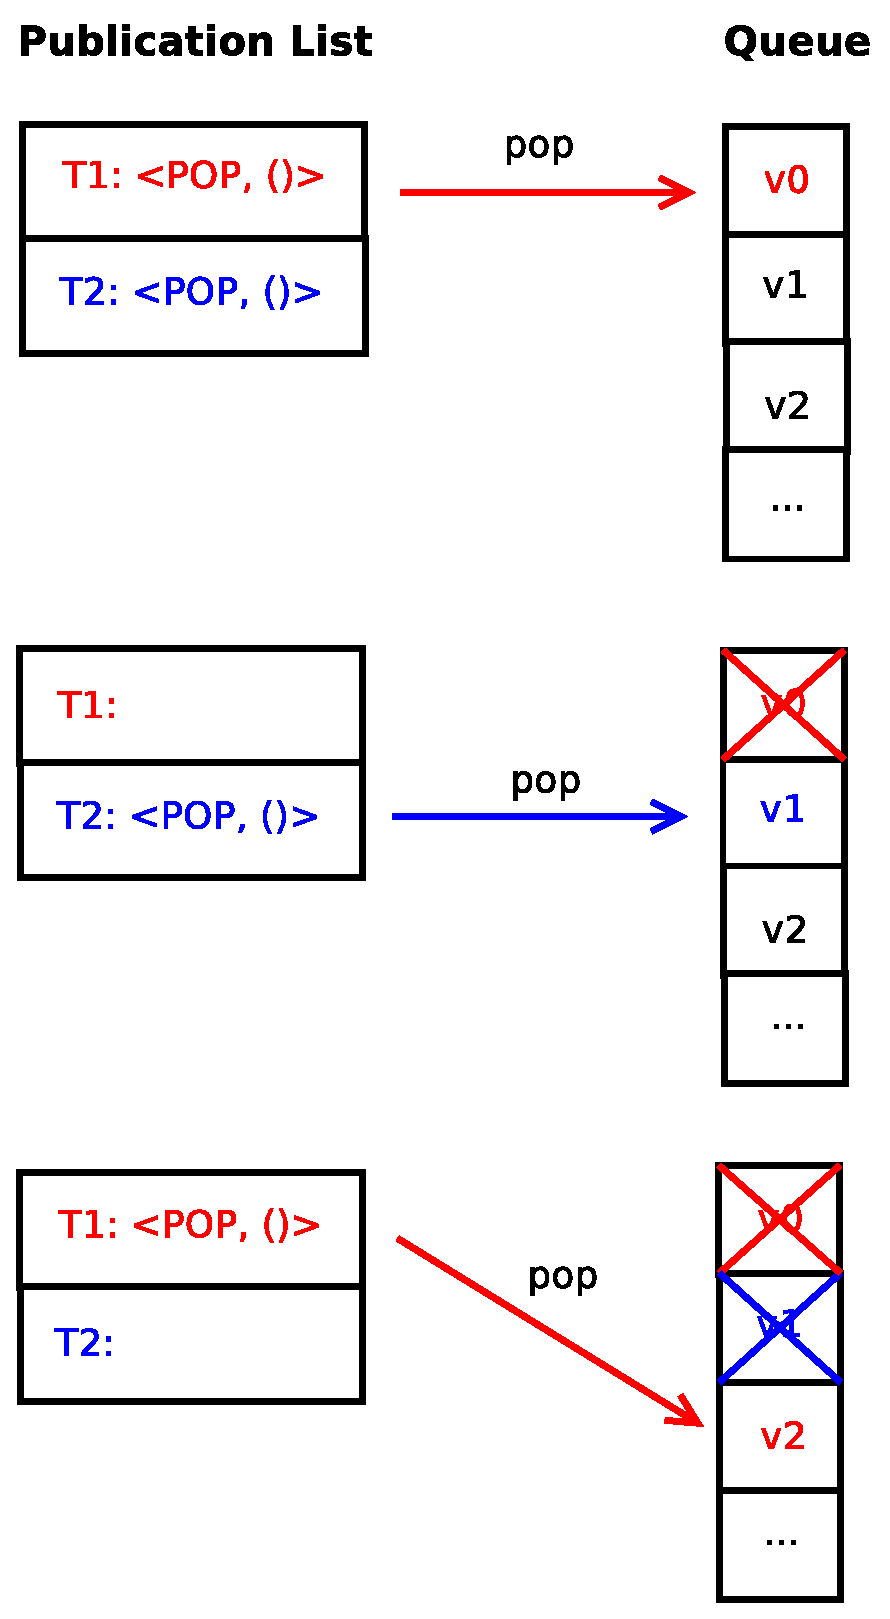
\includegraphics[width=0.45\textwidth]{fcqueue_publist}
\caption{Invalid order of pop application in the flat combining queue.}
\label{fig:fcqueue_publist}
\end{figure}

Recall that, in addition to the requirements for a correct concurrent queue, a transactional queue must guarantee that there exists a serial order of all transactions such that, within one transaction, any two pops pop consecutive values in the queue starting from the head of the queue and any two pushes push consecutive values at the tail of the queue.
This means that we must consider the order in which threads' requests are applied to the queue to be able to create a transactionally correct flat combining queue. For example, let a transaction in thread T1 be \texttt{\{pop, pop\}} and a transaction in thread T2 be \texttt{\{pop\}}. The combiner thread sees that T1 has published \texttt{<POP,()>} and T2 has published \texttt{<POP,()>} to the publication list. The combiner thread then applies \texttt{T1:Pop} (popping the head of the queue) and \texttt{T2:Pop} (popping the second item on the queue). When the next combining pass executes, the combiner thread will see that T1 has published \texttt{<POP,()>} again to the queue. However, performing T1's second pop violates the queue's transactional specification: the two popped values in T1's transaction will not be consecutive. This sequence is shown in Figure~\ref{fig:fcqueue_publist}. T1 must now abort, which means that T2's pop becomes invalid: it popped the second-frontmost value of the queue, rather than the head of the queue.

Detecting these invalid orderings requires two important changes to flat combining (we describe the rationale for these changes in Chapter~\ref{commutativity}): 
\begin{enumerate}
\item A push cannot be applied to the queue during a transaction's execution, and must instead be performed when a transaction commits.
\item An uncommitted pop in a thread's transaction must be unobservable by any other thread. This can be implemented in two ways:  
    \begin{enumerate}
        \item The algorithm can delay a transaction's pops until commit time. This then means the algorithm must track which values in the queue are going to be popped within the transaction. This prevents duplicate pops and detects if the queue will be ``empty'' by tracking how many values will be popped off the queue during this transaction. If another thread performs a pop or push during the transaction's lifetime, this can cause the transaction to abort: the ``empty'' status of the queue at commit time may now be inconsistent with what the transaction saw during execution. 
        \item The algorithm does not execute flat combining requests from other threads until the transaction has committed or aborted (a pessimistic approach). Because only this thread can execute commands, pops can be performed at execution time (and restored to the head of the queue if the transaction aborts). This can be implemented either by aborting the other threads' transactions or by forcing the other threads to block or spin.
    \end{enumerate}
\end{enumerate}

We now describe the new algorithms for push and pop.  We change the types of request a thread can publish to its record on the publication list. Recall that the original flat combining queue supports two requests: \texttt{<PUSH, value>} and \texttt{<POP, ()>}. The transactional queue supports the follow requests:
\begin{itemize}
    \item \texttt{<PUSH, list>} : push a list of values onto the queue
    \item \texttt{<MARK\_POP, thread\_id>} : mark a value in the queue as ``to be popped'' by this \texttt{thread\_id}
    \item \texttt{<DEQ, thread\_id>} : dequeue all values in the queue that are marked ``to be popped'' by this \texttt{thread\_id}
    \item \texttt{<EMPTY?, thread\_id>} : check if the queue, after popping all items marked by this \texttt{thread\_id}, is empty
    \item \texttt{<CLEANUP, thread\_id>} : unmark all values that are marked with this \texttt{thread\_id}
\end{itemize}

As with the T-QueueO and T-QueueP, a push within a transaction adds to an internal \texttt{write\_list\_item}. At commit time, the thread will post a \texttt{<PUSH, list>} request with the \texttt{write\_list} passed as the argument.

A pop is implemented with a pessimistic approach. Performing a pop within a transaction invokes the \texttt{<MARK\_POP, thread\_id>} request. The combiner thread, upon seeing a \texttt{MARK\_POP} request, looks at the first value at the head of the queue. If this value is marked with another thread's \texttt{thread\_id}, the combiner thread returns \texttt{<ABORT>} to the calling thread. This scenario is shown in Figure~\ref{fig:fcqueue_abort1}.

\begin{figure}[t]
\centering
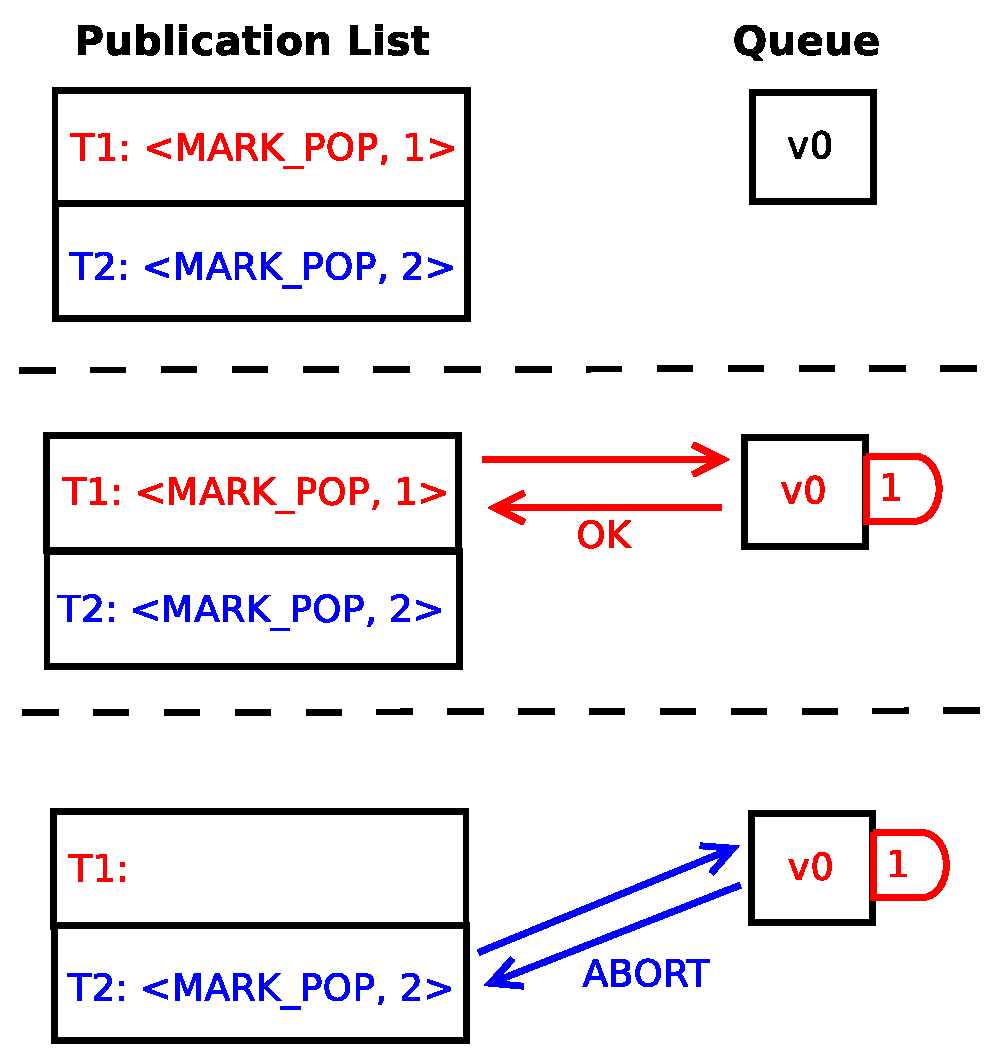
\includegraphics[width=0.45\textwidth]{fcqueue_abort1}
    \caption{Abort when calling \texttt{<MARK\_POP>} in the transactional flat combining queue.}
\label{fig:fcqueue_abort1}
\end{figure}

If the value is not marked, the combiner thread marks the value with the caller's \texttt{thread\_id} and returns \texttt{<OK>}. Note that in this scenario, no other thread will be able to mark values in the queue until the calling thread commits or aborts; other threads will abort when seeing the head value marked by the calling thread's \texttt{thread\_id}. 

If the value is neither marked by another thread nor unmarked, then the value must already be marked with this thread's \texttt{thread\_id}, and the combiner thread iterates sequentially through the queue values until it reaches a value not marked by the calling thread's \texttt{thread\_id}. It then marks the value with the caller's \texttt{thread\_id} and returns \texttt{<OK>}. Upon receiving the response, the calling thread adds a write to a \texttt{pop\_item} to tell the thread to post a \texttt{<DEQ, thread\_id>} request at commit time. This request will tell the combiner thread to actually remove the popped value from the queue.

If the queue is either empty or all values are marked with the caller's \texttt{thread\_id}, the combiner thread will return \texttt{<EMPTY>}, which is remembered by the calling thread. An \texttt{<EMPTY>} response requires that the size of the queue be checked at commit time.

Note that this algorithm does not allow pops to read the values pushed within the same transaction. To do so would require passing in the thread's \texttt{write\_list} in addition to the \texttt{thread\_id} as arguments to the combiner thread. During our evaluation, we leave this part of the transactional queue specification unimplemented (and note that adding \emph{read-my-writes} support will only decrease performance).

The \texttt{<EMPTY?, thread\_id>} request is posted at commit time when a thread tries to commit a transaction that observed an empty queue at some point in its execution. This happens when the thread receives an \texttt{<EMPTY>} response to a \texttt{<MARK\_POP>} request during the transaction. If \texttt{[<EMPTY?, thread\_id> == true]}, this implies that the queue state is currently empty.
The thread therefore knows that no other thread has pushed onto the queue since the time it saw an empty queue while performing a \texttt{<MARK\_POP>}, and it can safely commit the transaction. If \texttt{[<EMPTY?, thread\_id> == false]}, the queue is no longer empty---another thread has pushed items onto the queue---and this thread's \texttt{<MARK\_POP>} result is invalid. The transaction must therefore abort. This scenario is shown in Figure~\ref{fig:fcqueue_abort2}.

\begin{figure}[t]
\centering
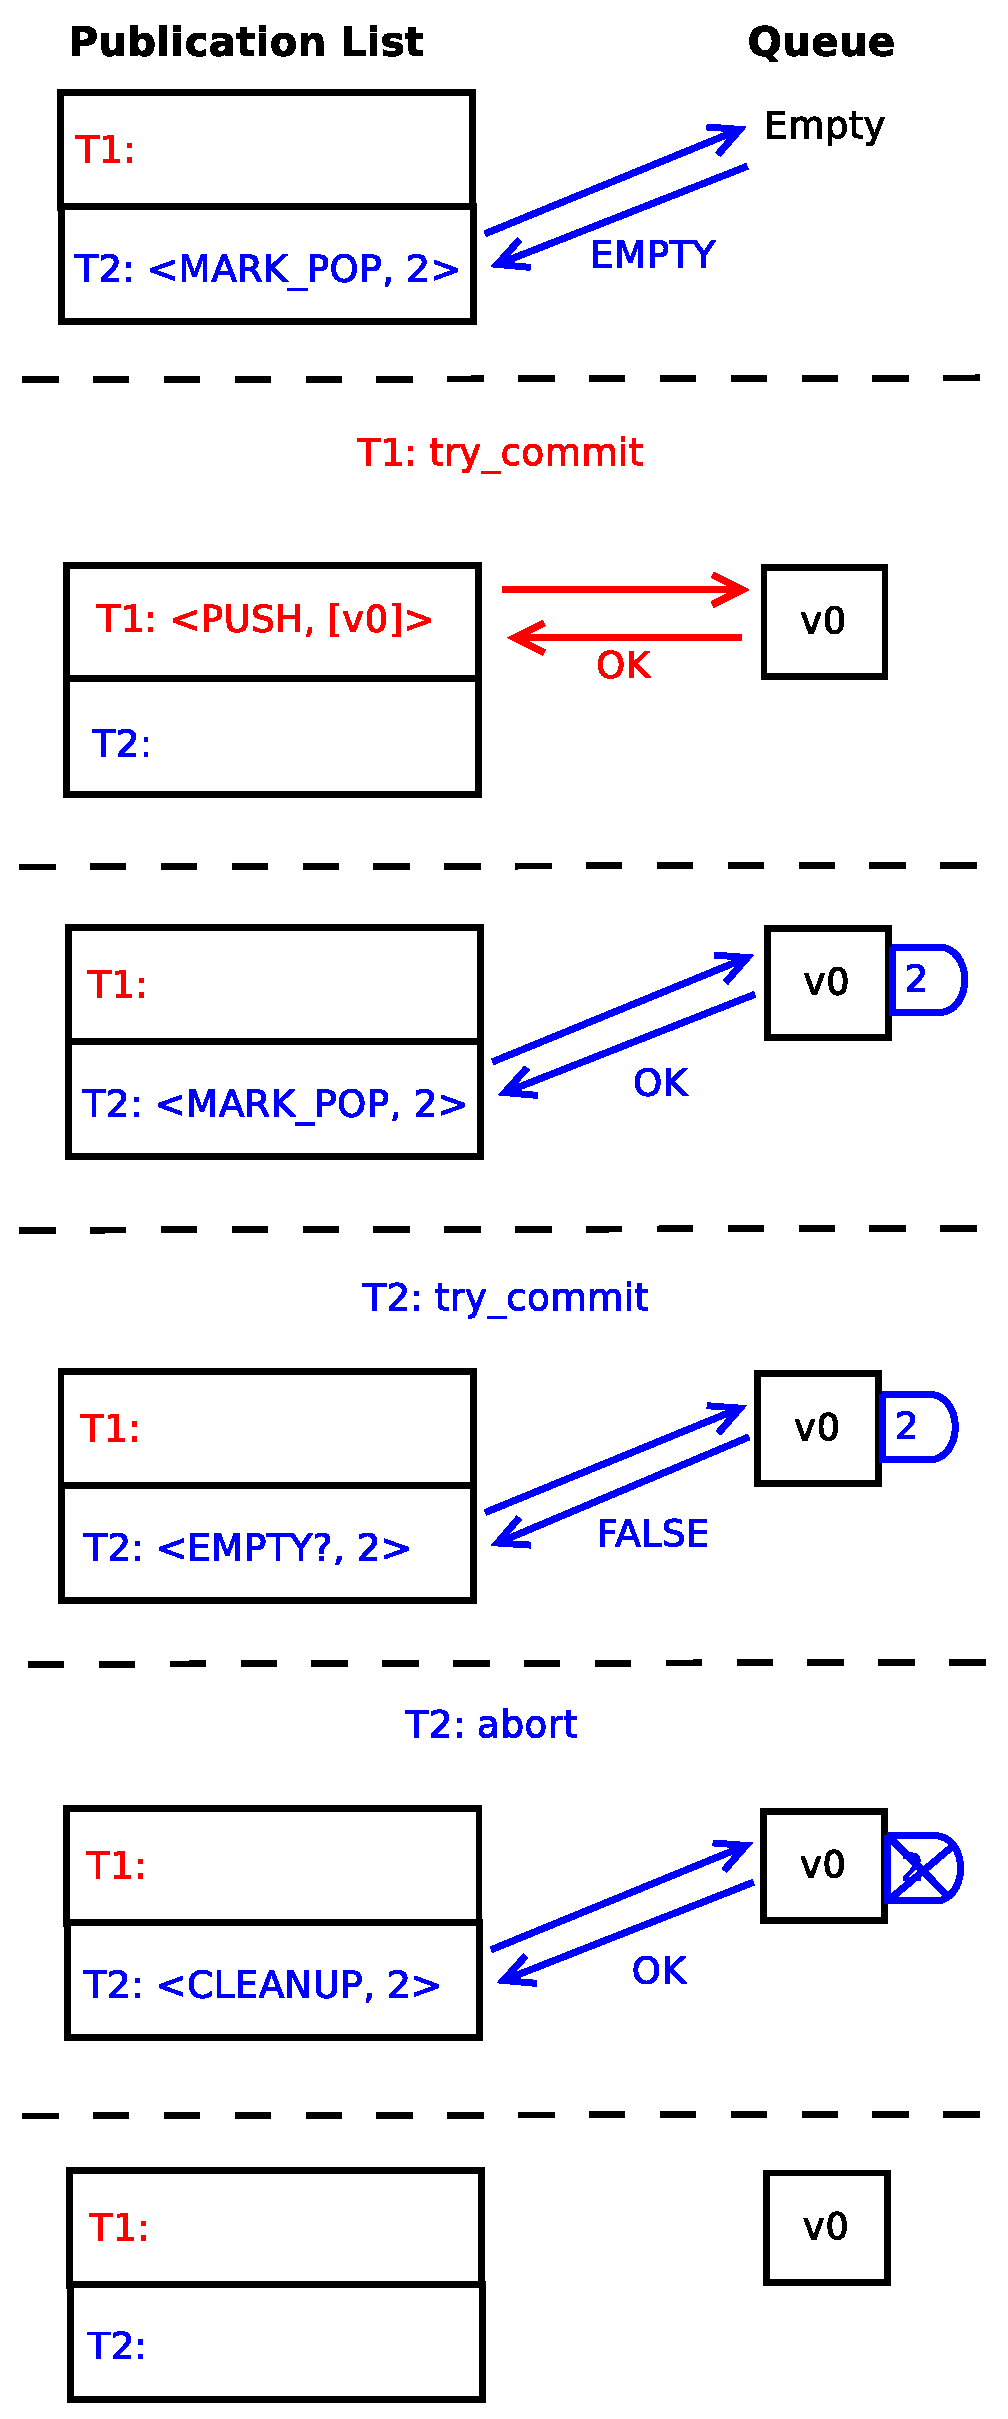
\includegraphics[width=0.45\textwidth]{fcqueue_abort2}
    \caption{Abort when checking \texttt{<EMPTY?>} in the transactional flat combining queue.}
\label{fig:fcqueue_abort2}
\end{figure}

If a thread ever sees an empty queue when executing a pop \emph{and} subsequently performs a push within the same transaction, the thread must prevent another transaction from committing between the time of the empty check and the installation of its pushed value. This requires adding what is essentially a lock of the tail of the queue. This is implemented via additional machinery in the combiner thread code, which signals whether or not a transaction has locked the queue and prevents any other thread's pushes from being installed until the ``lock'' is released.

The \texttt{<CLEANUP, thread\_id>} request is posted when a thread aborts a transaction and must unmark any items in the queue that it had marked as pending pops. The combiner thread iterates through the queue from the head and unmarks any items with the \texttt{thread\_id}.
